\documentclass[answers,dvipsnames]{exam}
\usepackage{marvosym}

%...TikZ & PGF
\usepackage{pgfplots}
\pgfplotsset{compat=1.11}
\tikzset{>=latex}
\usetikzlibrary{calc,math}
\usepackage{tikzsymbols}
\usepgfplotslibrary{fillbetween}
\usetikzlibrary{decorations.markings} 
\usetikzlibrary{arrows.meta} %...APP2 for arrows as objects and images
\usetikzlibrary{backgrounds} %...For shading portions of graphs
\usetikzlibrary{patterns} %...Unit 5 Problems
\usetikzlibrary{shapes.geometric} %...For drawing cylinders in Unit 2
\tikzset{
    mark position/.style args={#1(#2)}{
        postaction={
            decorate,
            decoration={
                markings,
                mark=at position #1 with \coordinate (#2);
            }
        }
    }
} %...See https://tex.stackexchange.com/questions/43960/define-node-at-relative-coordinates-of-draw-plot

\tikzset{
    declare function = {trajectoryequation10(\x,\vi,\thetai)= tan(\thetai)*\x - 10*\x^2/(2*(\vi*cos(\thetai))^2);},
    declare function = {trajectoryequation(\x,\vi,\thetai)= tan(\thetai)*\x - 9.8*\x^2/(2*(\vi*cos(\thetai))^2);},
    declare function = {patheq(\x,\yi,\vi,\thetai)= \yi + tan(\thetai)*\x - 9.8*\x^2/(2*(\vi*cos(\thetai))^2);},
    declare function = {patheqten(\x,\yi,\vi,\thetai)= \yi + tan(\thetai)*\x - 10*\x^2/(2*(\vi*cos(\thetai))^2);} %like patheq but with gravity = 10
}

%...siunitx
\usepackage{siunitx}
\DeclareSIUnit{\nothing}{\relax}
\def\mymu{\SI{}{\micro\nothing} }
\DeclareSIUnit\mmHg{mmHg}
\DeclareSIUnit{\mile}{mi}
%...NOTE: "The product symbol between the number and unit is set using the quantity-product option."

%...Other
\usepackage{amsthm}
\usepackage{amsmath}
\usepackage{amssymb}
\usepackage{cancel}
\usepackage{subcaption}
\usepackage{dashrule}
\usepackage{enumitem}
\usepackage{fontawesome}
\usepackage{multicol}
\usepackage{glossaries}
%\numberwithin{equation}{section}
\numberwithin{figure}{section}
\usepackage{float}
\usepackage{twemojis} %...twitter emojis
\usepackage{utfsym}
\newcommand{\R}{\mathbb{R}} %...real number symbol
\usepackage{graphicx}
\graphicspath{ {../Figures/} }
\usepackage{hyperref}
\hypersetup{colorlinks=true,
    linkcolor=blue,
    filecolor=magenta,
    urlcolor=cyan,}
\urlstyle{same}
\newcommand{\hdashline}{{\hdashrule{\textwidth}{0.5pt}{0.8mm}}}
\newcommand{\hgraydashline}{{\color{lightgray} \hdashrule{0.99\textwidth}{1pt}{0.8mm}}}

%...Miscellaneous user-defined symbols
\newcommand{\fnet}{F_{\text{net}}} %...For net force
\newcommand{\bvec}[1]{\vec{\mathbf{#1}}} %...bold vector
\newcommand{\bhat}[1]{\,\hat{\mathbf{#1}}} %...bold hat vector
\newcommand{\que}{\mathord{?}}  %...Question mark symbol in equation env
%...Define thick horizontal rule for examples:
\newcommand{\hhrule}{\hrule\hrule}
\let\oldtexttt\texttt% Store \texttt
\renewcommand{\texttt}[2][black]{\textcolor{#1}{\ttfamily #2}}% 

%...For use in the exam document class
\newif\ifprintmetasolutions


%...Decreases space above and below align and gather enironment
\makeatletter
\g@addto@macro\normalsize{%
  \setlength\abovedisplayskip{-3pt}
  \setlength\belowdisplayskip{6pt} 
}
\makeatother





\usepackage[margin=1in]{geometry}
\usepackage[figurewithin=none]{caption}
\usepackage{exam-randomizechoices}

\CorrectChoiceEmphasis{\color{red}\bfseries}
\renewcommand{\solutiontitle}{\noindent\textbf{\textcolor{red}{Solution:}}\enspace}

\usepackage{OutilsGeomTikz}
\usepackage{utfsym} %...Symbols in Unit 7 Problems
\usepackage{tabu} %...Symbols in Unit 7 Problems

%...For use in Unit 2            %    
\setlength{\columnsep}{2cm}      %
\setlength{\columnseprule}{1pt}  %
\usepackage[none]{hyphenat}      %
%%%%%%%%%%%%%%%%%%%%%%%%%%%%%%%%%

%...For use in Unit 11 on Waves:
\pgfdeclarehorizontalshading{visiblelight}{50bp}{  %
color(0.00000000000000bp)=(red);                   %
color(8.33333333333333bp)=(orange);                %
color(16.66666666666670bp)=(yellow);               %
color(25.00000000000000bp)=(green);                %
color(33.33333333333330bp)=(cyan);                 %
color(41.66666666666670bp)=(blue);                 %
color(50.00000000000000bp)=(violet)                %
}                                                  %

\newcommand{\checkbox}[1]{%
  \ifnum#1=1
    \makebox[0pt][l]{\raisebox{0.15ex}{\hspace{0.1em}\Large$\checkmark$}}%
  \fi
  $\square$%
}
%%%%%%%%%%%%%%%%%%%%%%%%%%%%%%%%%%%%%%%%%%%%%%%%%%%%

%...If using circuitikz package:
% \ctikzset{bipoles/battery1/height=0.5}
% \ctikzset{bipoles/battery1/width=0.25}
% \ctikzset{bipoles/resistor/height=0.15}
% \ctikzset{bipoles/resistor/width=0.4}

\setrandomizerseed{1}

\firstpageheader{Physics}{Unit 6: One-Dimensional Motion}{Summative Assessment}
\runningheader{}{}{}

\begin{document}
\begin{questions}

\question 
Hugo throws a ball straight down off a cliff. One second later his friend, Arthur, throws a ball straight up. Which velocity vs time graph below could depict the motion of Hugo’s ball in the scenario given?

\begin{center}
    \begin{tikzpicture}
        \draw[->] (0,-1.25) -- ++(0,2.5) node[above,rotate=90,pos=0.5] {$v$ (m/s)};
        \draw[->] (0,0) -- ++(2.5,0) node[below,pos=0.9] {$t$ (s)};
        \draw[thick,red] (0,1) -- ++(1.5,-2);
        \node at (1.25,1.5) {\textbf{Graph A}};
    \end{tikzpicture}
    \hspace{2em}
    \begin{tikzpicture}
        \draw[->] (0,-1.25) -- ++(0,2.5) node[above,rotate=90,pos=0.5] {$v$ (m/s)};
        \draw[->] (0,0) -- ++(2.5,0) node[below,pos=0.9] {$t$ (s)};
        \draw[thick,red] (0.6,1) -- ++(1.5,-2);
        \node at (1.25,1.5) {\textbf{Graph B}};
    \end{tikzpicture}
    \hspace{2em}
    \begin{tikzpicture}
        \draw[->] (0,-1.25) -- ++(0,2.5) node[above,rotate=90,pos=0.5] {$v$ (m/s)};
        \draw[->] (0,0) -- ++(2.5,0) node[below,pos=0.9] {$t$ (s)};
        \draw[thick,red] (0,0) -- ++(0.75,-1);
        \node at (1.25,1.5) {\textbf{Graph C}};
    \end{tikzpicture}
    \hspace{2em}
    \begin{tikzpicture}
        \draw[->] (0,-1.25) -- ++(0,2.5) node[above,rotate=90,pos=0.5] {$v$ (m/s)};
        \draw[->] (0,0) -- ++(2.5,0) node[below,pos=0.9] {$t$ (s)};
        \draw[thick,red] (0,-0.5) -- ++(0.38,-0.7);
        \node at (1.25,1.5) {\textbf{Graph D}};
    \end{tikzpicture}
\end{center}

\begin{randomizechoices}[norandomize]
    \choice Graph A
    \choice Graph B
    \choice Graph C
    \correctchoice Graph D
\end{randomizechoices}

\question
A car is moving at \SI{20}{m/s} when the driver spots a deer in the road. He brakes to come to a complete stop in 15 seconds.  What is the distance the car traveled once the driver started braking?

\begin{randomizechoices}[norandomize]
    \choice \SI{35}{m}
    \correctchoice \SI{150}{m}
    \choice \SI{300}{m}
    \choice \SI{1.33}{m}
\end{randomizechoices}

\question
A \SI{20}{kg} rock sits on the edge of a \SI{80}{m} high cliff.  What would the final velocity of the rock be if it is dropped from the edge of the cliff?

\begin{randomizechoices}[norandomize]
    \choice \SI{1600}{m/s}
    \choice \SI{30}{m/s}
    \correctchoice \SI{40}{m/s}
    \choice \SI{20}{m/s}
\end{randomizechoices}

\question
The following time and velocity data was collected for a ball that was launched across a rough surface. 

\begin{center}
    \begin{tabular}{|c|c|}
        \hline
        \textbf{Time} (s) & \textbf{Velocity} (m/s) \\ \hline
        0 & 0.55\\ \hline
        1 & 0.45\\ \hline
        2 & 0.35\\ \hline
        3 & 0.25\\ \hline
        4 & 0.15\\ \hline
    \end{tabular}
\end{center}

Using the information above, determine the acceleration of the ball. 

\begin{randomizechoices}[norandomize]
    \correctchoice \SI{-0.10}{m/s^2}
    \choice \SI{-0.55}{m/s^2}
    \choice \SI{-0.35}{m/s^2}
    \choice \SI{-0.15}{m/s^2}
\end{randomizechoices}

\question 
What is the acceleration of the car from 0 seconds to 4 seconds?

\begin{center}
    \begin{tikzpicture}
        \begin{axis}[width=6cm,
            height=6cm,
            xmin=0,xmax=6,
            ymin=0,ymax=15,
            xlabel={Time (s)},
            ylabel={Velocity (m/s)},
            xtick={0,2,...,6},
            ytick={0,5,...,15},
            minor tick num=1,
            grid=both,
            ]
            \addplot[black,very thick]
                coordinates{(0,0)(4,10)(6,10)};
        \end{axis}
    \end{tikzpicture}
\end{center}

\begin{randomizechoices}[norandomize]
    \choice \SI{10}{m/s^2}
    \choice \SI{0.0}{m/s^2}
    \correctchoice \SI{2.5}{m/s^2}
    \choice \SI{2.0}{m/s^2}
\end{randomizechoices}

\question
As an object is moving upwards, what is true about the object’s motion? \textbf{Select 2 answers.}

\begin{center}
    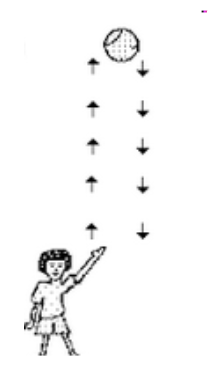
\includegraphics[height=3cm]{physics/figures/figure-unit-5-ball-in-the-air.png}
\end{center}

\begin{randomizechoices}[norandomize]
    \choice The velocity and acceleration are both decreasing.
    \choice Positive work is being done by the force of gravity on the object.
    \correctchoice Impulse from the force of gravity is causing the ball’s velocity to decrease.
    \correctchoice The velocity and acceleration are in opposite directions.
\end{randomizechoices}

\question
A rock is dropped from a cliff of the same height on the earth (\SI{9.8}{m/s^2}) and on Jupiter (\SI{25}{m/s^2}). Which will take longer to fall to the ground? On Earth or Jupiter?

\begin{randomizechoices}[norandomize]
    \choice Neither because both cliffs are the same height.
    \choice Neither, it will fall the same on both planets because gravitational acceleration doesn’t matter.
    \correctchoice Earth because the gravitational acceleration is smaller.
    \choice Jupiter because the gravitational acceleration is larger. 
\end{randomizechoices}

\question
When an object is released from rest and falls freely to the ground, what two quantities do we know?

\begin{randomizechoices}[norandomize]
    \choice final velocity \& acceleration
    \choice initial velocity \& final velocity
    \choice time \& velocity
    \correctchoice initial velocity \& acceleration
\end{randomizechoices}

\question 
An object moving vertically that has negative acceleration and a negative velocity is:

\begin{randomizechoices}[norandomize]
    \choice Moving Upwards
    \correctchoice Moving Downwards
    \choice At the top of its motion
    \choice Not enough info to tell
\end{randomizechoices}

\begin{EnvUplevel}
    Compare the motion of the three rocks below. Select the choice that best answer the questions below. Answer choices may be used more than once.
\end{EnvUplevel}

\begin{center}
    \begin{tabular}{|c|l|}
        \hline 
        \textbf{Option A} & A \SI{5}{kg} rock is thrown upwards from a \SI{10}{m} cliff\\ \hline
        \textbf{Option B} & A \SI{10}{kg}  rock is thrown downwards from a \SI{10}{m} cliff\\ \hline
        \textbf{Option C} & A \SI{5}{kg} rock is dropped from a \SI{10}{m} cliff\\ \hline
        \textbf{Option D} &  All rocks considered equal\\ \hline
    \end{tabular}
\end{center}

\question
Which rock(s) will hit the ground in the shortest amount of time?

\begin{randomizechoices}[norandomize]
    \choice Option A
    \correctchoice Option B
    \choice Option C
    \choice Option D
\end{randomizechoices}

\question
Which rock(s) will have the greatest acceleration?

\begin{randomizechoices}[norandomize]
    \choice Option A
    \choice Option B
    \choice Option C
    \correctchoice Option D
\end{randomizechoices}


\question
Which rock(s) will have both a positive and negative slope on a position time graph?

\begin{randomizechoices}[norandomize]
    \correctchoice Option A
    \choice Option B
    \choice Option C
    \choice Option D
\end{randomizechoices}

\question
Which rock(s) will reach the highest point?

\begin{randomizechoices}[norandomize]
    \correctchoice Option A
    \choice Option B
    \choice Option C
    \choice Option D
\end{randomizechoices}


\question
Which rock(s) will have the smallest Kinetic Energy when striking the ground?

\begin{randomizechoices}[norandomize]
    \choice Option A
    \choice Option B
    \correctchoice Option C
    \choice Option D
\end{randomizechoices}

\begin{EnvUplevel}
    Compare the motion of the four objects below. Select the choice that best answers the question. Answers may be used more than once. 
\end{EnvUplevel}

\begin{center}
    \begin{tabular}{|c|l|}
        \hline 
        \textbf{Option A} & A \SI{5}{kg} object thrown at \SI{10}{m/s} upwards from a \SI{10}{m} cliff\\ \hline
        \textbf{Option B} & A \SI{5}{kg} object thrown at \SI{10}{m/s} upwards from a \SI{20}{m} cliff\\ \hline
        \textbf{Option C} & All objects considered equal\\ \hline
    \end{tabular}
\end{center}

\question
Which object(s) has the greatest momentum at the highest point of it’s motion?

\begin{randomizechoices}[norandomize]
    \choice Option A
    \choice Option B
    \correctchoice Option C
\end{randomizechoices}


\question
Which object(s) will experience the greatest net work from the force of gravity during it’s motion?

\begin{randomizechoices}[norandomize]
    \choice Option A
    \correctchoice Option B
    \choice Option C
\end{randomizechoices}


\question
Which object(s) will experience the greatest impulse from the force of gravity during its motion?

%...NOTE: According to the answer key of the teacher who made this question, the answer to this question should be Option A.

\begin{randomizechoices}[norandomize]
    \choice Option A %...Answer key says this is the right answer. But I don't see how?
    \correctchoice Option B
    \choice Option C
\end{randomizechoices}



\question
Which object(s) will have the greatest final velocity when striking the ground?

\begin{randomizechoices}[norandomize]
    \choice Option A
    \correctchoice Option B
    \choice Option C
\end{randomizechoices}

\question
Answer the questions that follow. The initial velocity of a \SI{3}{kg} ball sent upward from the ground, is \SI{12}{m/s}. 


\begin{center}
    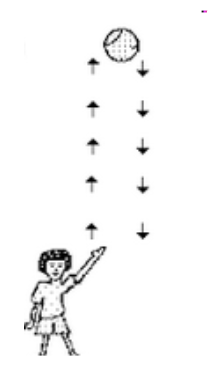
\includegraphics[width=3cm]{physics/figures/figure-unit-5-ball-in-the-air.png}
\end{center}

\begin{parts}
    \part What is the total distance the the ball travels? Be sure to show all work.

    \begin{solution}
        \SI{14.4}{m}
    \end{solution}
    
    \part Use kinematics to find the time to the highest point. Be sure to show all work.

    \begin{solution}
        \SI{1.2}{s}
    \end{solution}
    
    \part Use the impulse-momentum theorem to find the time to the highest point. Be sure to show all work.

    \begin{solution}
        \SI{1.2}{s}
    \end{solution}
\end{parts}

\clearpage
\printkeytable
\bigskip

\textbf{NOTE:} Question 6 has 2 correct answers. Only one of the them is shown in the table above.



\end{questions}
\end{document}
